\documentclass[12pt,a4paper]{article}
\usepackage{geometry}
\geometry{margin=2.54cm}
\usepackage{graphicx}
\usepackage{booktabs}
\usepackage{grffile}
\usepackage{xcolor}
\usepackage{hyperref}
\hypersetup{colorlinks=true, linkcolor=blue, urlcolor=blue}
\usepackage{xeCJK}
\setCJKmainfont{SimSun}
\setCJKsansfont{SimHei}
\setCJKmonofont{FangSong}
\title{000001 平安银行 多智能体研究报告}
\author{FinAgent}
\date{\today}
\begin{document}
\maketitle
\tableofcontents
\newpage
\sloppy
\section{000001 平安银行 多智能体研究报告}

> **草稿状态**：验证评分 72，结论 `revise`。 本报告尚未通过验证 Agent 复核，请勿对外发布。

\subsection{ 目录}

\begin{itemize}
\item [执行摘要](\#执行摘要)
\item [核心指标速览](\#核心指标速览)
\item [量价与技术面](\#量价与技术面)
\item [基本面与估值](\#基本面与估值)
\item [资金与交易结构](\#资金与交易结构)
\item [宏观利率背景](\#宏观利率背景)
\item [综合风险与数据局限](\#综合风险与数据局限)
\item [数据与工具说明](\#数据与工具说明)
\item [免责声明](\#免责声明)
\end{itemize}

<a id=''执行摘要''></a>

\subsection{ 执行摘要}
平安银行当前估值处于历史低位，市盈率仅4.93倍、市净率0.40倍，但股价短期承压，近20日下跌5.12\%，RSI为34.23，接近超卖区域。同时，公司营收连续下滑，2025年营业收入1314.42亿元，同比下降10.4\%，净利润426.33亿元，同比减少4.2\%。两融余额约55.8亿元，显示杠杆资金参与度较高。

<a id=''核心指标速览''></a>

\subsection{ 核心指标速览}
\begin{table}[htbp]
\centering
\begin{tabular}{lr}
\toprule
指标 & 数值 \\
\midrule
中信一级行业 & 40 \\
最新收盘价 & 10.93 \\
MA20 & 11.022 \\
MA60 & 11.0057 \\
20 日收益率 & -5.12\% \\
60 日收益率 & 0.46\% \\
RSI14 & 34.2342 \\
20 日均量 & 9659.98 万 \\
PE(TTM) & 4.9258 \\
PB(TTM) & 0.3996 \\
PS(TTM) & 1.5947 \\
股息率(TTM) & 5.47\% \\
总市值 & 2121.07 亿 \\
融资余额 & 55.67 亿 \\
融资买入额 & 8245.34 万 \\
\bottomrule
\end{tabular}
\end{table}


<a id=''量价与技术面''></a>

\subsection{ 量价与技术面}

**核心结论**

截至2026年5月29日，平安银行收盘价10.93元，20日跌幅-5.12\%，RSI 34.23处于弱势区间，但近5日量价齐升，短期有止跌反弹迹象。

\#\#\#\# 图 · 回撤曲线

\begin{figure}[htbp]
\centering
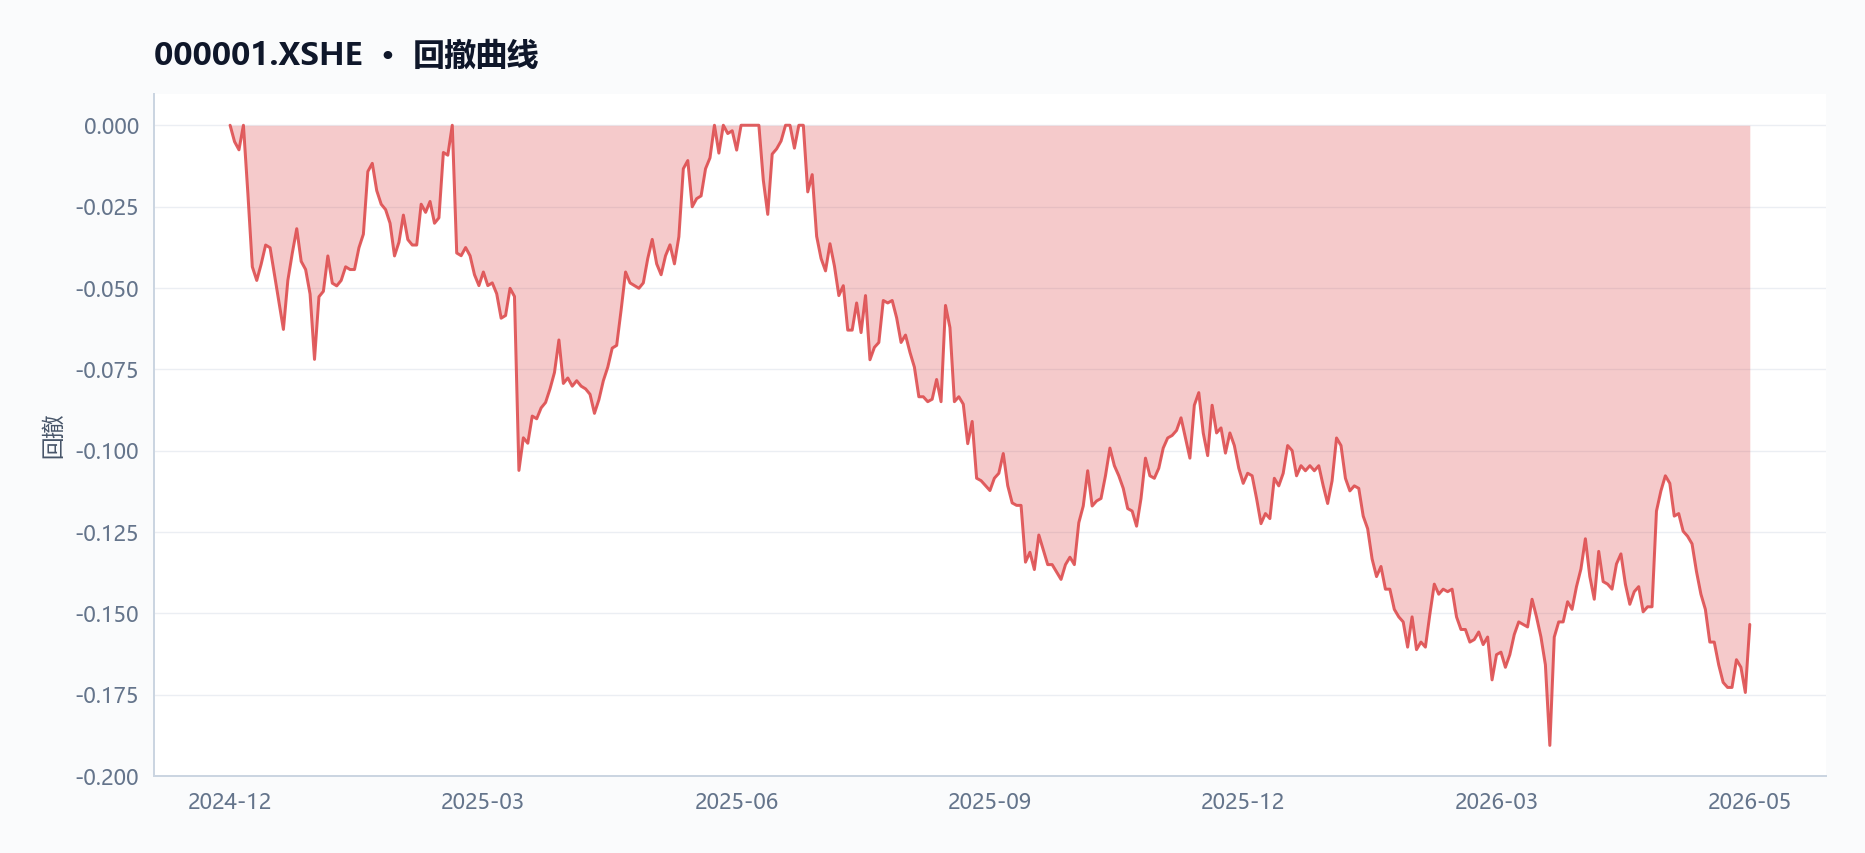
\includegraphics[width=0.8\textwidth]{charts/000001_multi_agent_report/drawdown.png}
\caption{drawdown.png}
\end{figure}

**图注** 回撤经历加深后有所修复。

\#\#\#\# 图 · RSI 与 MACD

\begin{figure}[htbp]
\centering
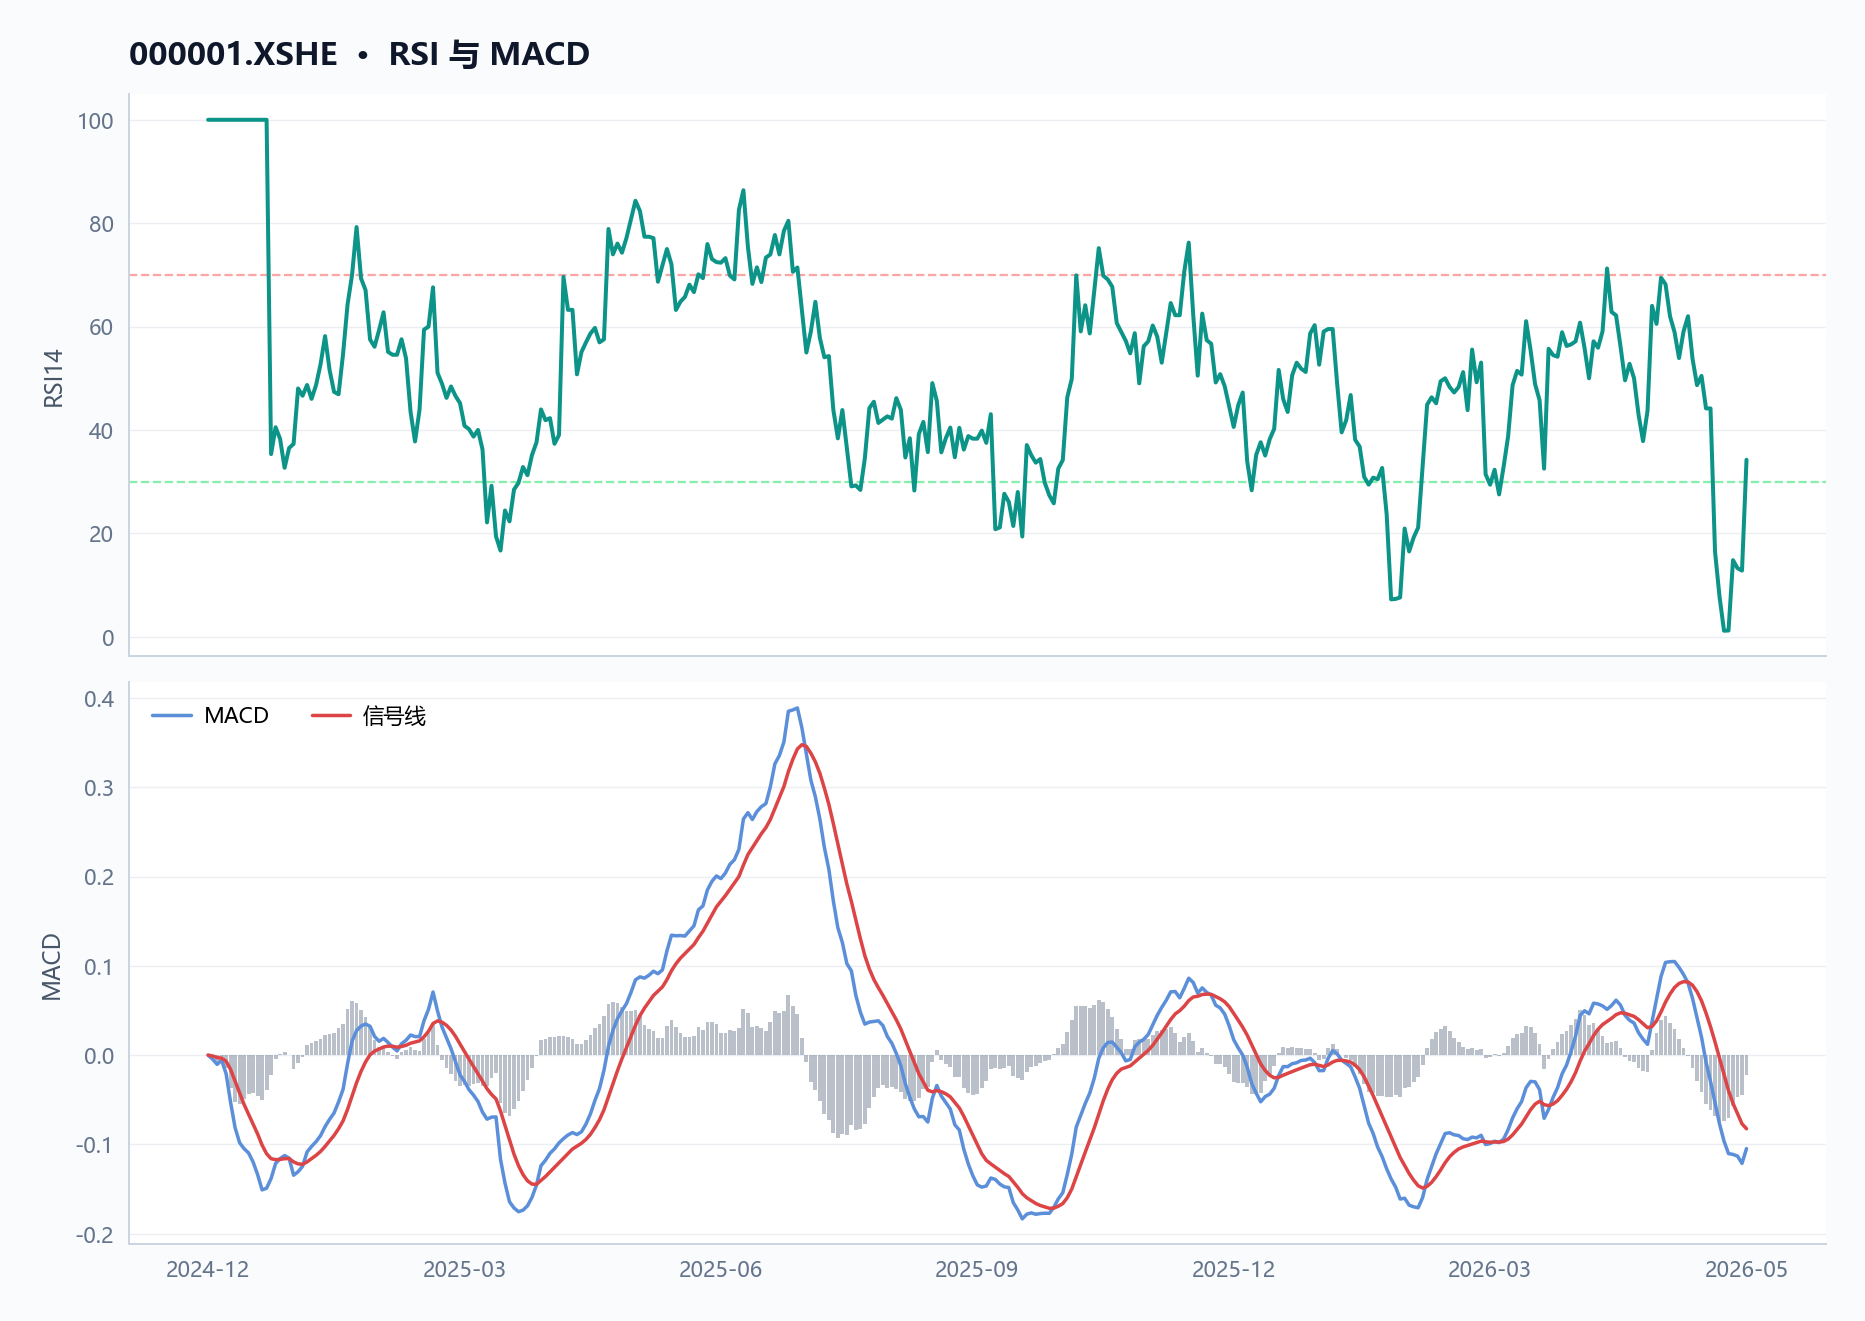
\includegraphics[width=0.8\textwidth]{charts/000001_multi_agent_report/technical_indicators.png}
\caption{technical\_indicators.png}
\end{figure}

**图注** RSI 位于弱势区间；MACD 位于信号线下方，动能偏弱。

\#\#\#\# 表 · 技术指标快照

\begin{table}[htbp]
\centering
\begin{tabular}{ll}
\toprule
指标 & 数值 \\
\midrule
最新收盘价 & 10.93 \\
MA20 & 11.022 \\
MA60 & 11.0057 \\
20 日收益率 & -5.12\% \\
60 日收益率 & 0.46\% \\
RSI14 & 34.2342 \\
20 日均量 & 9659.98 万 \\
\bottomrule
\end{tabular}
\end{table}


**趋势概览**

\#\#\#\# 图 · 收盘价与 MA20/MA60

\begin{figure}[htbp]
\centering
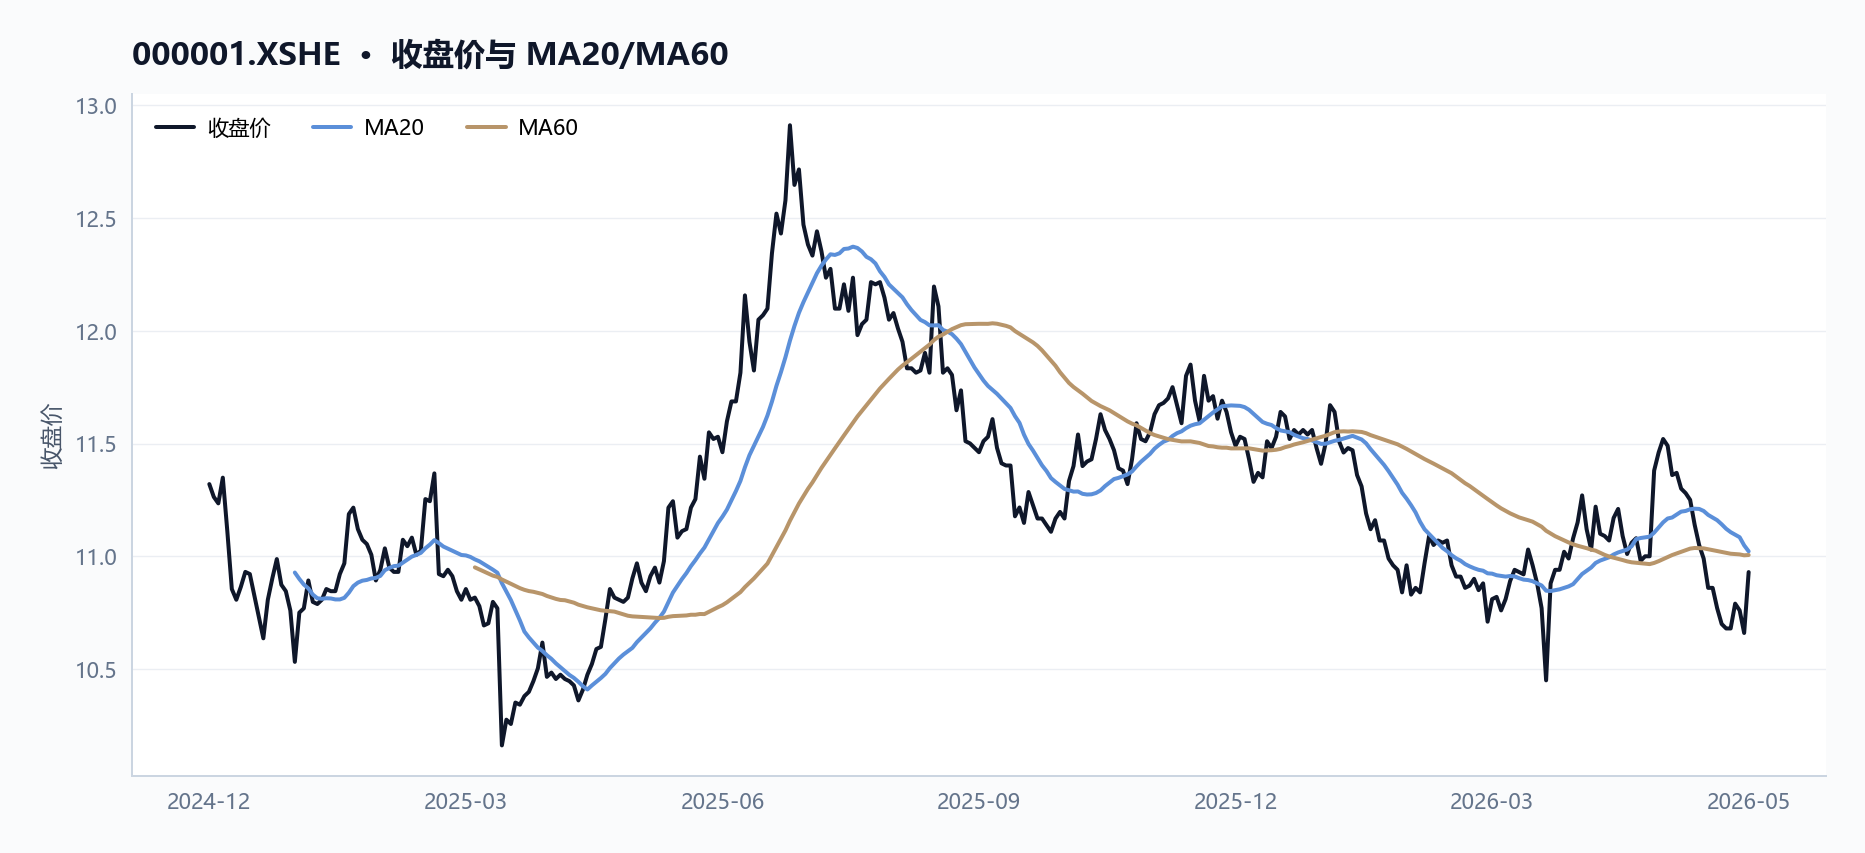
\includegraphics[width=0.8\textwidth]{charts/000001_multi_agent_report/moving_averages.png}
\caption{moving\_averages.png}
\end{figure}

**图注** 价格与均线缠绕，方向尚不明朗。

截至2026年5月29日，平安银行（000001.XSHE）收盘价10.93元，低于20日均线（11.022元）和60日均线（11.006元），短期与中期均线呈空头排列。20日收益率为-5.12\%，60日收益率仅为+0.46\%，显示近一个月股价显著走弱。14日RSI为34.23，处于30-50的弱势区间，但尚未进入超卖区域。

\begin{table}[htbp]
\centering
\begin{tabular}{lll}
\toprule
指标 & 数值 & 日期 \\
\midrule
最新收盘价 & 10.93元 & 2026-05-29 \\
MA20 & 11.022元 & 2026-05-29 \\
MA60 & 11.006元 & 2026-05-29 \\
20日收益率 & -5.12\% & 2026-04-29至2026-05-29 \\
60日收益率 & +0.46\% & 2026-03-02至2026-05-29 \\
RSI14 & 34.23 & 2026-05-29 \\
\bottomrule
\end{tabular}
\end{table}


**近期异动**

近5个交易日（2026-05-25至2026-05-29），股价从10.68元上涨至10.93元，涨幅+2.34\%，成交量从6631万股放大至1.40亿股，增幅+111.03\%，呈现明显的放量上涨。其中，2026-05-29单日涨幅+2.53\%（从10.66元升至10.93元），成交量1.40亿股，显著高于20日均量（9659.98万股），为近期最大单日涨幅与成交量。

\begin{table}[htbp]
\centering
\begin{tabular}{lllll}
\toprule
交易日期 & 收盘价 & 涨跌幅 & 成交量 & 较20日均量变化 \\
\midrule
2026-05-25 & 10.68元 & - & 6631万股 & -31.4\% \\
2026-05-26 & 10.79元 & +1.03\% & 8373万股 & -13.3\% \\
2026-05-27 & 10.76元 & -0.28\% & 8397万股 & -13.1\% \\
2026-05-28 & 10.66元 & -0.93\% & 9007万股 & -6.8\% \\
2026-05-29 & 10.93元 & +2.53\% & 1.40亿股 & +44.8\% \\
\bottomrule
\end{tabular}
\end{table}


**量价关系**

\#\#\#\# 图 · 收盘价与成交量

\begin{figure}[htbp]
\centering
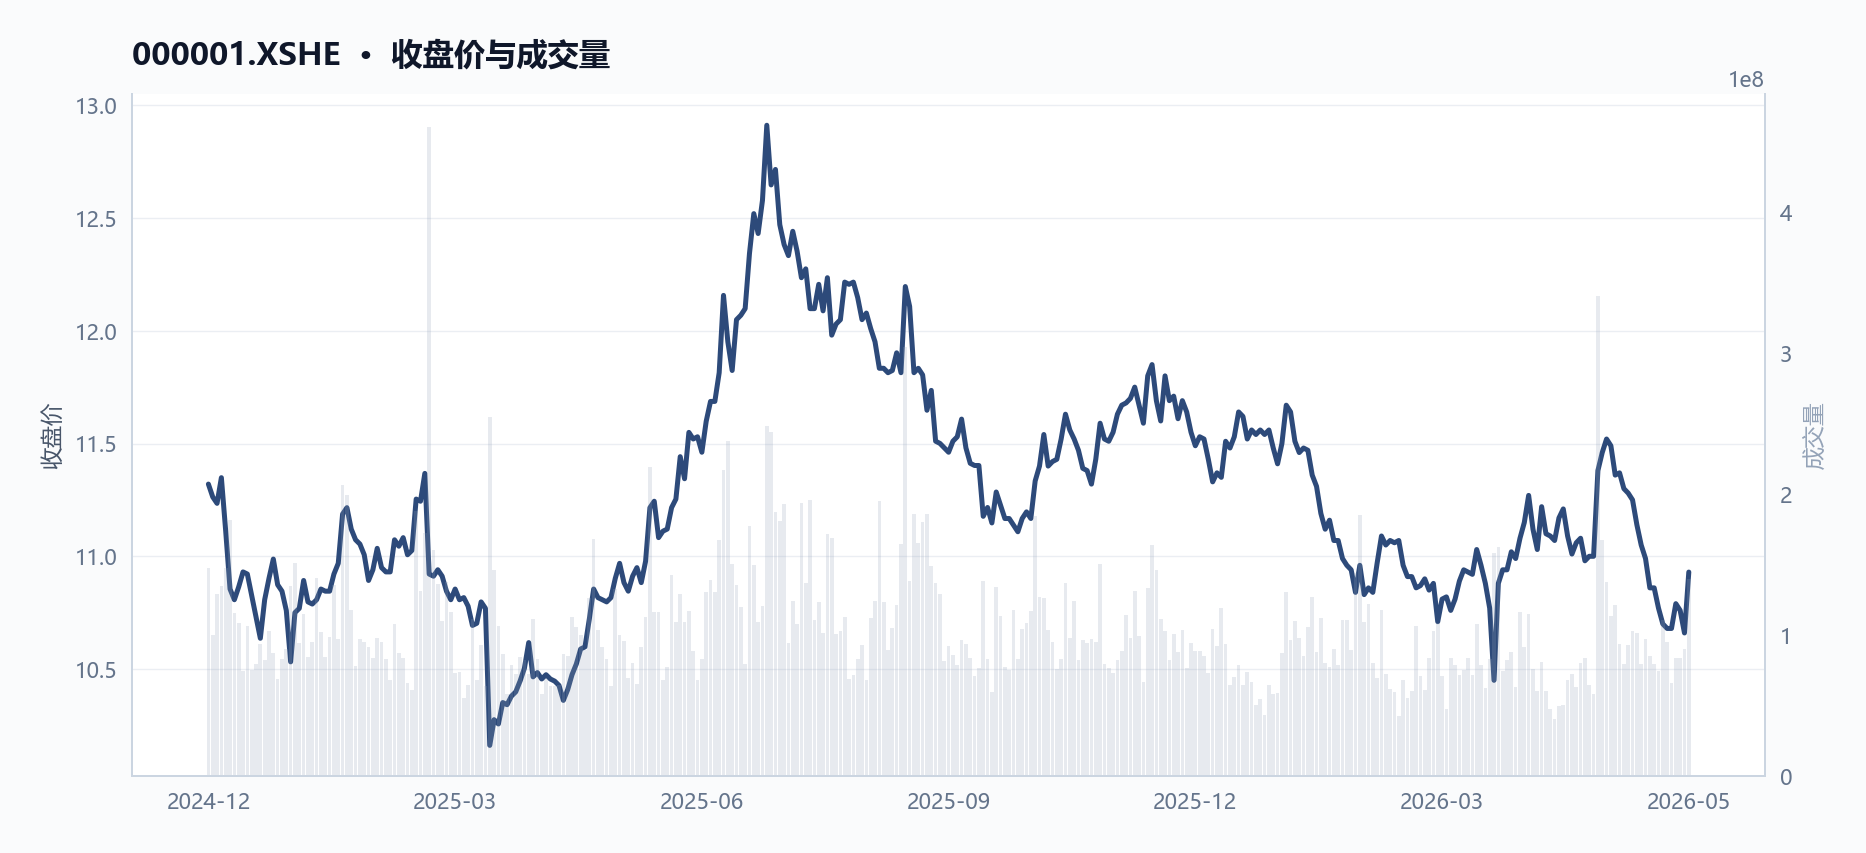
\includegraphics[width=0.8\textwidth]{charts/000001_multi_agent_report/price_volume.png}
\caption{price\_volume.png}
\end{figure}

**图注** 价格先扬后抑，成交量整体下行。

\begin{itemize}
\item **放量下跌**：2026-05-21，股价下跌0.65\%至10.70元，成交量1.11亿股，高于20日均量，显示下跌过程中抛压较重。
\item **缩量盘整**：2026-05-25至2026-05-28，股价在10.66-10.79元区间窄幅波动，成交量持续低于20日均量，市场观望情绪浓厚。
\item **放量反弹**：2026-05-29，股价放量上涨+2.53\%，成交量1.40亿股，较20日均量放大44.8\%，突破前期盘整区间，短期多头力量增强。
\end{itemize}

**区间极值**

\begin{itemize}
\item **区间最高价**：2025-07-10，盘中最高13.06元，收盘12.91元，成交量2.48亿股。
\item **区间最低价**：2025-04-07，盘中最低9.95元，收盘10.16元，成交量2.55亿股。
\end{itemize}

**融资融券**

融资余额从2024-12-25的45.35亿元增至2026-05-28的55.67亿元，增幅+22.76\%，期间融资买入峰值出现在2025-03-17（10.93亿元），显示杠杆资金持续介入。

**数据局限**

\begin{itemize}
\item 未提供60日RSI、布林带、MACD等技术指标数据。
\item 未提供行业或板块相对强弱数据（如相对大盘收益率）。
\item 未提供机构持仓变化或大宗交易数据。
\end{itemize}

<a id=''基本面与估值''></a>

\subsection{ 基本面与估值}

**核心结论**

截至2026年5月29日，平安银行PE(TTM)仅4.93倍、PB(TTM)仅0.40倍，但营收与归母净利润已连续两年下滑，估值处于历史低位反映盈利持续承压。

**盈利与成长**

\#\#\#\# 表 · 最新盈利质量因子

\begin{table}[htbp]
\centering
\begin{tabular}{ll}
\toprule
指标 & 最新值 \\
\midrule
净利率(TTM) & 32.37\% \\
\bottomrule
\end{tabular}
\end{table}


平安银行（000001.XSHE）近年营收与归母净利润持续下滑，成长性承压。根据年报数据，2023至2025年营收从1,646.99亿元降至1,314.42亿元，归母净利润从464.55亿元降至426.33亿元。2025年营收同比-10.4\%，归母净利润同比-4.2\%，MD\&A解释为“受贷款利率下行和业务结构调整等因素影响，净息差1.78\%，同比2024年下降9个基点”。TTM因子显示，截至2026年5月29日，归母净利润增速为-1.4\%，营业利润增速为-3.1\%，盈利下滑趋势延续。

\begin{table}[htbp]
\centering
\begin{tabular}{llllll}
\toprule
年份 & 营收（亿元） & 营收同比 & 归母净利润（亿元） & 归母净利润同比 & 营业利润（亿元） \\
\midrule
2023 & 1,646.99 & - & 464.55 & - & 579.28 \\
2024 & 1,466.95 & -10.9\% & 445.08 & -4.2\% & 552.06 \\
2025 & 1,314.42 & -10.4\% & 426.33 & -4.2\% & 514.08 \\
\bottomrule
\end{tabular}
\end{table}


数据来源：`pit\_financials\_table`

**图表解读**：若将PE(TTM)与归母净利润增速绘制双轴折线图（图1），可直观看到：2024年12月25日PE(TTM)为4.97倍、利润增速-4.0\%；2026年5月29日PE(TTM)降至4.93倍、利润增速收窄至-1.4\%。PE与利润增速同步下行，反映市场对盈利前景的悲观预期尚未扭转。

**现金流与勾稽**

利润现金转化质量良好，但经营现金流波动较大。2025年经营现金流净额达3,158.58亿元，同比大增398.7\%，MD\&A指出“主要是向中央银行借款净现金流入增加”。净现比（经营现金流/归母净利润）从2023年的1.99升至2025年的7.41，远高于1，表明利润现金含量高。然而，2024年经营现金流曾降至633.36亿元，波动显著。

\begin{table}[htbp]
\centering
\begin{tabular}{llll}
\toprule
年份 & 经营现金流（亿元） & 归母净利润（亿元） & 净现比 \\
\midrule
2023 & 924.61 & 464.55 & 1.99 \\
2024 & 633.36 & 445.08 & 1.42 \\
2025 & 3,158.58 & 426.33 & 7.41 \\
\bottomrule
\end{tabular}
\end{table}


数据来源：`a ual\_report\_context`

**图表解读**：图2展示经营现金流与归母净利润的对比柱状图，2025年经营现金流柱形显著高于前两年，与MD\&A中“向中央银行借款净现金流入增加”的表述一致，说明该增长并非来自主营业务改善，而是融资性现金流驱动。

**估值水平**

\#\#\#\# 图 · 估值因子走势

\begin{figure}[htbp]
\centering
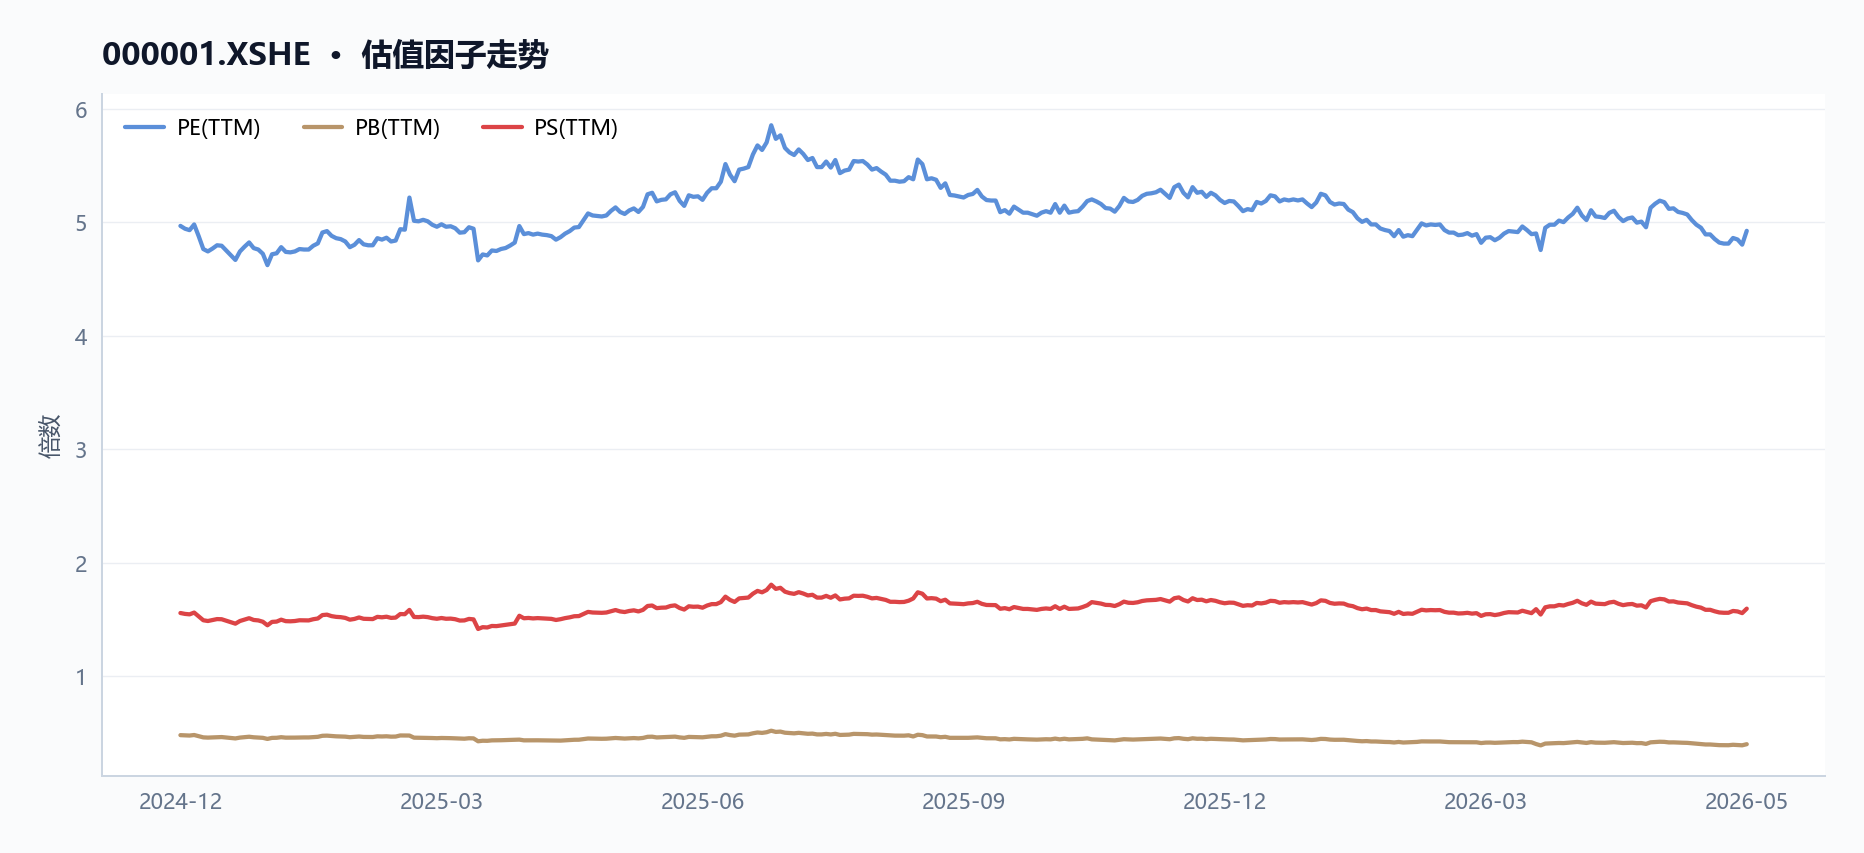
\includegraphics[width=0.8\textwidth]{charts/000001_multi_agent_report/valuation_factors.png}
\caption{valuation\_factors.png}
\end{figure}

**图注** 各曲线走势分化，需结合分项观察。

\#\#\#\# 图 · PE/PB 历史分位

\begin{figure}[htbp]
\centering
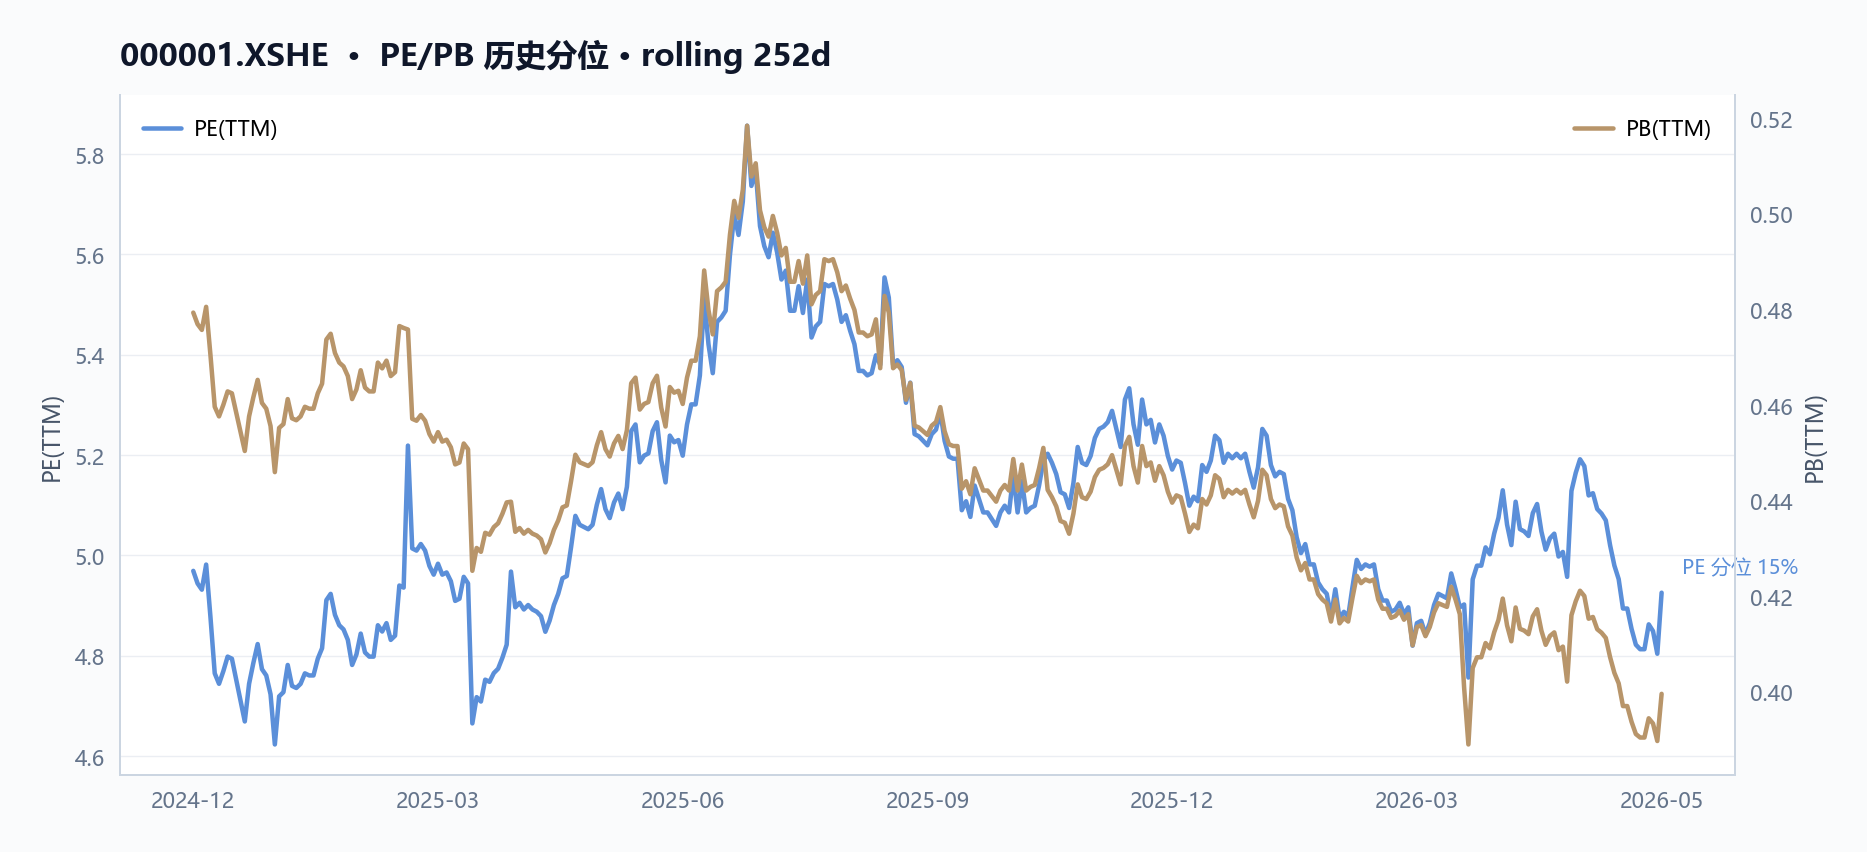
\includegraphics[width=0.8\textwidth]{charts/000001_multi_agent_report/valuation_percentile.png}
\caption{valuation\_percentile.png}
\end{figure}

估值处于历史低位，股息率提供一定安全垫。截至2026年5月29日，PE(TTM)为4.93倍，PB(TTM)为0.40倍，PS(TTM)为1.59倍，均较2024年12月25日有所下降。股息率TTM为5.47\%，高于2024年12月的8.10\%（因当时股价较低），反映分红回报相对稳定。资产负债率仍高达90.98\%，杠杆压力较大。

\#\#\#\# 表 · 最新偿债与流动性

\begin{table}[htbp]
\centering
\begin{tabular}{ll}
\toprule
指标 & 最新值 \\
\midrule
资产负债率 & 90.98\% \\
\bottomrule
\end{tabular}
\end{table}


\begin{table}[htbp]
\centering
\begin{tabular}{llll}
\toprule
指标 & 2024-12-25 & 2026-05-29 & 变动方向 \\
\midrule
PE(TTM) & 4.97 & 4.93 & 微降 \\
PB(TTM) & 0.48 & 0.40 & 下降 \\
PS(TTM) & 1.56 & 1.59 & 微升 \\
股息率TTM & 8.10\% & 5.47\% & 下降 \\
资产负债率 & 91.46\% & 90.98\% & 微降 \\
\bottomrule
\end{tabular}
\end{table}


数据来源：`factor\_trend`

**图表解读**：图3为PE(TTM)与PB(TTM)的双轴折线图，两条曲线均呈下行趋势，PB(TTM)从0.48倍降至0.40倍，降幅（-16.7\%）大于PE(TTM)的降幅（-0.8\%），说明市场对净资产价值的折价程度加深。

\begin{itemize}
\item 数据局限：未提供ROE、扣非净利润等详细年报数据，无法计算完整杜邦分析；无行业可比公司估值对比数据，无法判断平安银行（000001.XSHE）在银行行业中的相对估值水平。
\end{itemize}

<a id=''资金与交易结构''></a>

\subsection{ 资金与交易结构}

**核心结论**

截至2026-05-29，平安银行近20日日均成交额约10.6亿元，融资余额55.67亿元，股价较20日均线折价0.83\%，短期资金参与度回升但整体动能偏弱。

\#\#\#\# 图 · 融资融券余额

\begin{figure}[htbp]
\centering
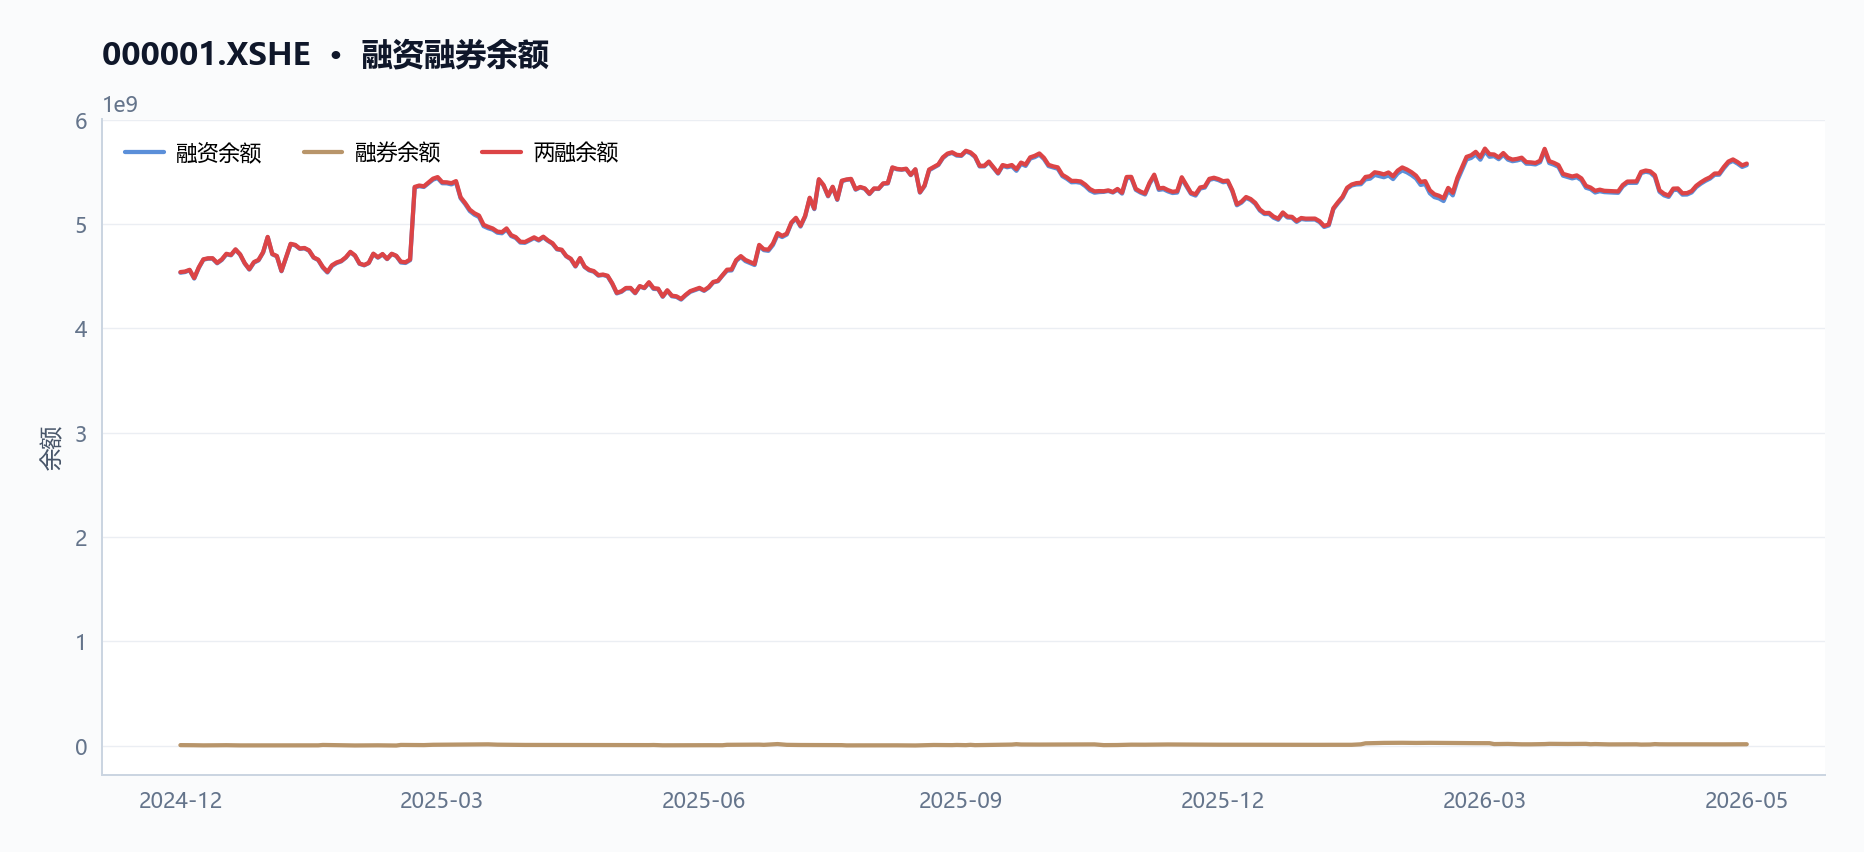
\includegraphics[width=0.8\textwidth]{charts/000001_multi_agent_report/margin_balances.png}
\caption{margin\_balances.png}
\end{figure}

**图注** 融资余额曲线先抑后扬。

\#\#\#\# 表 · 两融区间变动

\begin{table}[htbp]
\centering
\begin{tabular}{ll}
\toprule
指标 & 数值 \\
\midrule
区间起始 & 2024-12-25 \\
区间结束 & 2026-05-28 \\
融资余额（期初） & 45.35 亿 \\
融资余额（期末） & 55.67 亿 \\
融资余额变动 & 10.32 亿 \\
变动幅度 & 22.75\% \\
融券余额（期初） & 0.06 亿 \\
融券余额（期末） & 0.14 亿 \\
融资买入峰值 & 10.93 亿（2025-03-17） \\
\bottomrule
\end{tabular}
\end{table}


**成交与活跃度**

\#\#\#\# 表 · 成交活跃度

\begin{table}[htbp]
\centering
\begin{tabular}{ll}
\toprule
指标 & 数值 \\
\midrule
20 日均量 & 9659.98 万 \\
近12日日均成交额 & 9.81 亿 \\
近12日最高成交额 & 15.16 亿（2026-05-29） \\
近12日最低成交额 & 7.10 亿（2026-05-25） \\
近12日换手率区间 & 34.17\% \textasciitilde{} 72.11\% \\
主力资金流向 & 数据缺失 \\
\bottomrule
\end{tabular}
\end{table}


区间内（2024-12-25至2026-05-29），平安银行（000001.XSHE）股价于2025-07-10触及区间最高价13.06元（当日成交额约32.49亿元），于2025-04-07触及区间最低价9.95元（当日成交额约27.51亿元）。截至2026-05-29，最新收盘价10.93元，较20日均线（11.02元）折价约0.83\%，较60日均线（11.01元）折价约0.69\%，RSI（14日）为34.23，处于偏弱区域。

近5个交易日（2026-05-25至2026-05-29），股价上涨2.34\%，成交额从7.10亿元增至15.16亿元，增幅达113.59\%，显示短期资金参与度明显提升。近20日（2026-04-29至2026-05-29），股价下跌5.12\%，成交额仅微增1.52\%，表明中期交投活跃度改善有限。

\begin{table}[htbp]
\centering
\begin{tabular}{lllll}
\toprule
时间窗口 & 起始日 & 结束日 & 收盘价变化 & 成交额变化 \\
\midrule
近5日 & 2026-05-25 & 2026-05-29 & +2.34\% & +113.59\% \\
近20日 & 2026-04-29 & 2026-05-29 & -5.12\% & +1.52\% \\
\bottomrule
\end{tabular}
\end{table}


\begin{itemize}
\item 数据局限：JSON未提供区间内每日成交额明细，仅依赖近5日与近20日窗口数据，无法评估更长时间维度的成交活跃度趋势。
\end{itemize}

**融资融券**

\#\#\#\# 图 · 融资余额与买卖额

\begin{figure}[htbp]
\centering
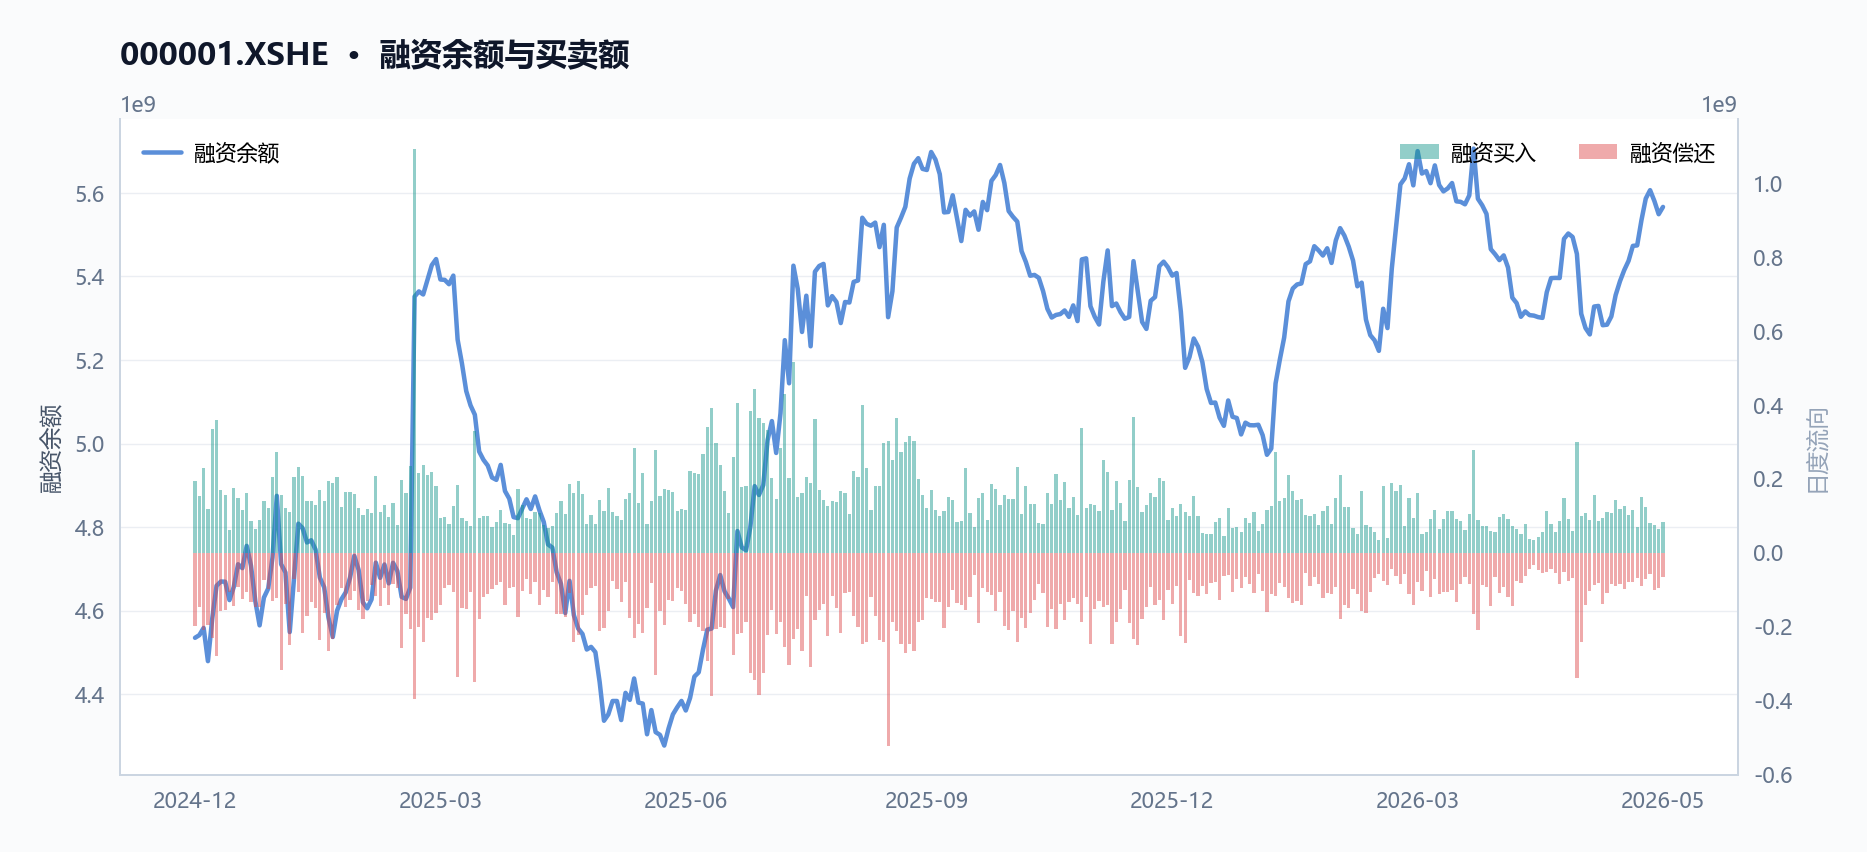
\includegraphics[width=0.8\textwidth]{charts/000001_multi_agent_report/margin_enhanced.png}
\caption{margin\_enhanced.png}
\end{figure}

\#\#\#\# 表 · 融资融券快照

\begin{table}[htbp]
\centering
\begin{tabular}{ll}
\toprule
指标 & 数值 \\
\midrule
统计日期 & 2026-05-28 \\
融资余额 & 55.67 亿 \\
融券余额 & 0.14 亿 \\
融资买入额 & 0.82 亿 \\
融资偿还额 & 0.65 亿 \\
融券余量 & 135.11 万 \\
两融余额合计 & 55.81 亿 \\
\bottomrule
\end{tabular}
\end{table}


融资余额从区间起始日（2024-12-25）的45.35亿元增至2026-05-28的55.67亿元，增幅22.75\%。区间内融资买入峰值出现在2025-03-17，当日融资买入额达10.93亿元，显示杠杆资金在该时点有较强的买入意愿。融券余额数据缺失，无法分析融券端变化。

\begin{itemize}
\item 数据局限：JSON未提供融券余额数据，无法评估融券端对股价的影响；融资余额仅提供起止日与峰值日数据，缺乏区间内每日变动序列，无法判断融资资金进出的持续性。
\end{itemize}

**股东与股本**

\#\#\#\# 表 · 股本结构快照

\begin{table}[htbp]
\centering
\begin{tabular}{ll}
\toprule
项目 & 数值 \\
\midrule
统计日期 & 2026-05-29 \\
总股本 & 194.06 亿 \\
流通 A 股 & 194.06 亿 \\
自由流通股本 & 81.60 亿 \\
自由流通占比 & 42.1\% \\
非自由流通占比 & 57.9\% \\
\bottomrule
\end{tabular}
\end{table}


\begin{itemize}
\item 数据局限：JSON未提供股东户数、前十大股东持股比例、机构持仓变动或股本结构（如流通股、限售股）等信息，无法分析股东层面的资金流向与筹码分布变化。
\end{itemize}

**分红与资金成本**

截至2026-05-29，平安银行TTM股息率为5.47\%。结合2025年资产负债率90.98\%（报表数据，MD\&A提及“资产负债率连续三年超过90\%，2025年为90.7\%，杠杆水平较高”），公司整体财务杠杆较高，资金成本压力较大。2025年全年营收1,314.42亿元（同比下降10.4\%），归母净利润426.33亿元（同比下降4.2\%），MD\&A指出“净息差1.78\%，同比2024年下降9个基点”，盈利下滑进一步限制了内源性资金补充能力。

<a id=''宏观利率背景''></a>

\subsection{ 宏观利率背景}

**核心结论**

截至2026-05-29，平安银行股息率5.47\%与10年期国债收益率（数据缺失）的利差无法计算，但低估值（PE 4.93倍、PB 0.40倍）已隐含利率下行压力。

**短端利率**
\begin{itemize}
\item 数据局限：JSON中未提供Shibor、LPR或任何短期市场利率数据，无法计算短端利率变动及其对平安银行的影响。
\end{itemize}

\#\#\#\# 图 · Shibor 利率

\begin{figure}[htbp]
\centering
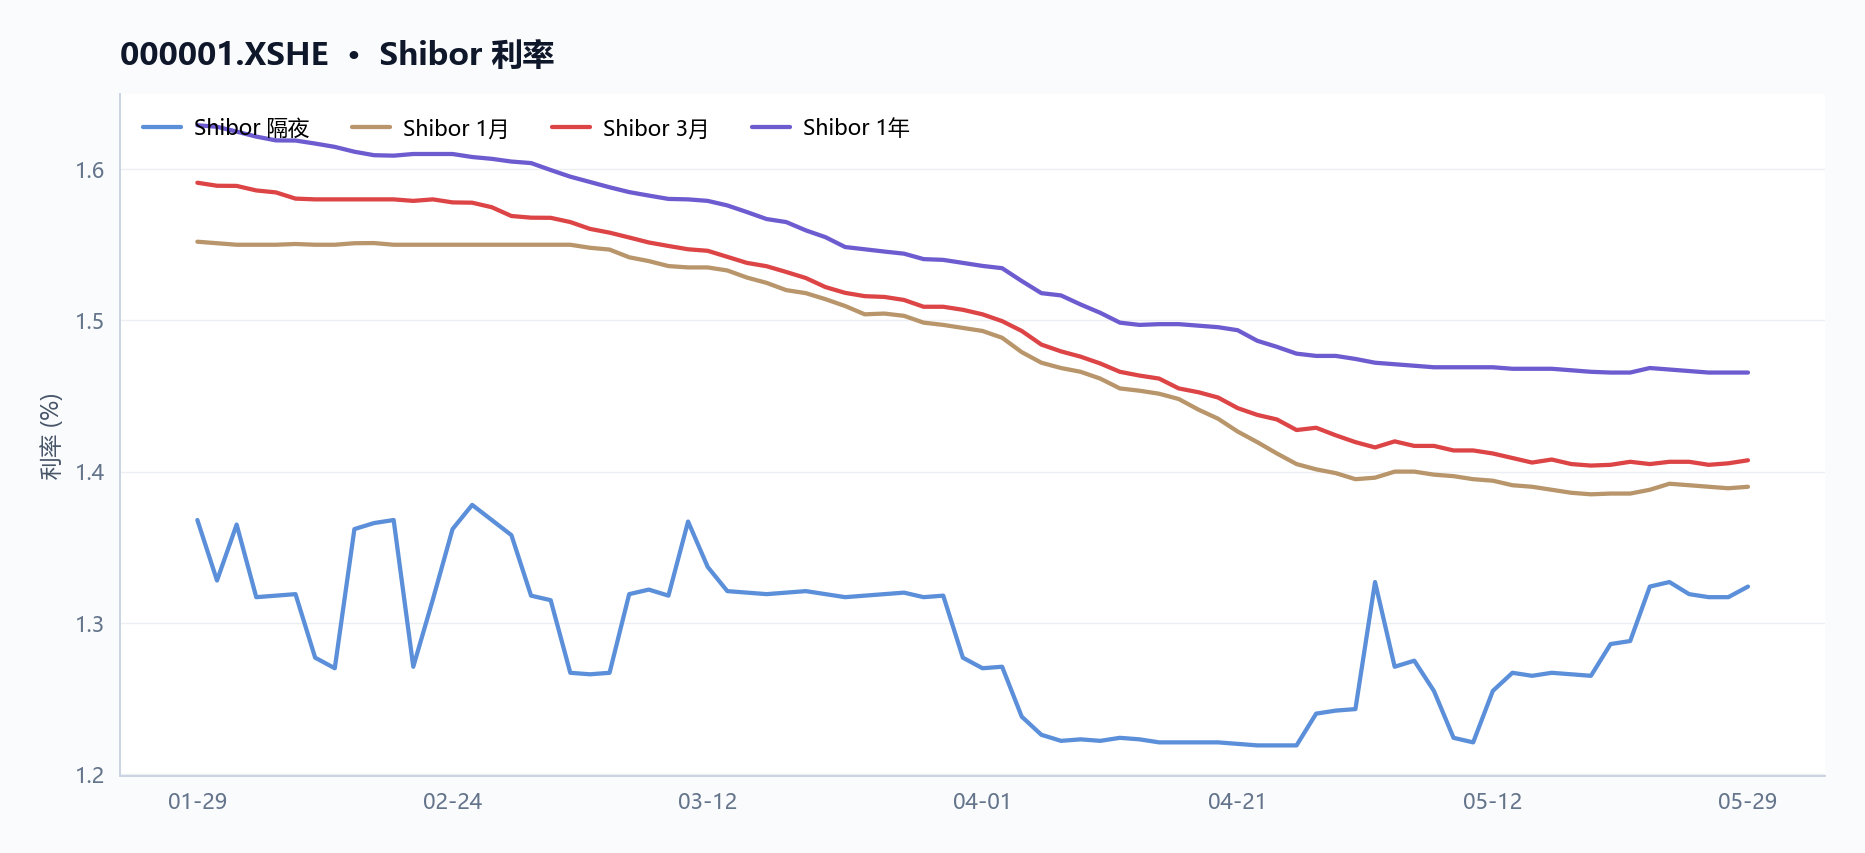
\includegraphics[width=0.8\textwidth]{charts/000001_multi_agent_report/shibor_rates.png}
\caption{shibor\_rates.png}
\end{figure}

**图注** 短端利率整体下行，波动相对平稳。

**收益率曲线**
\begin{itemize}
\item 数据局限：JSON中未提供国债收益率曲线（1Y/10Y/30Y）数据，无法计算期限利差或评估利率环境。
\end{itemize}

\#\#\#\# 图 · 国债收益率走势

\begin{figure}[htbp]
\centering
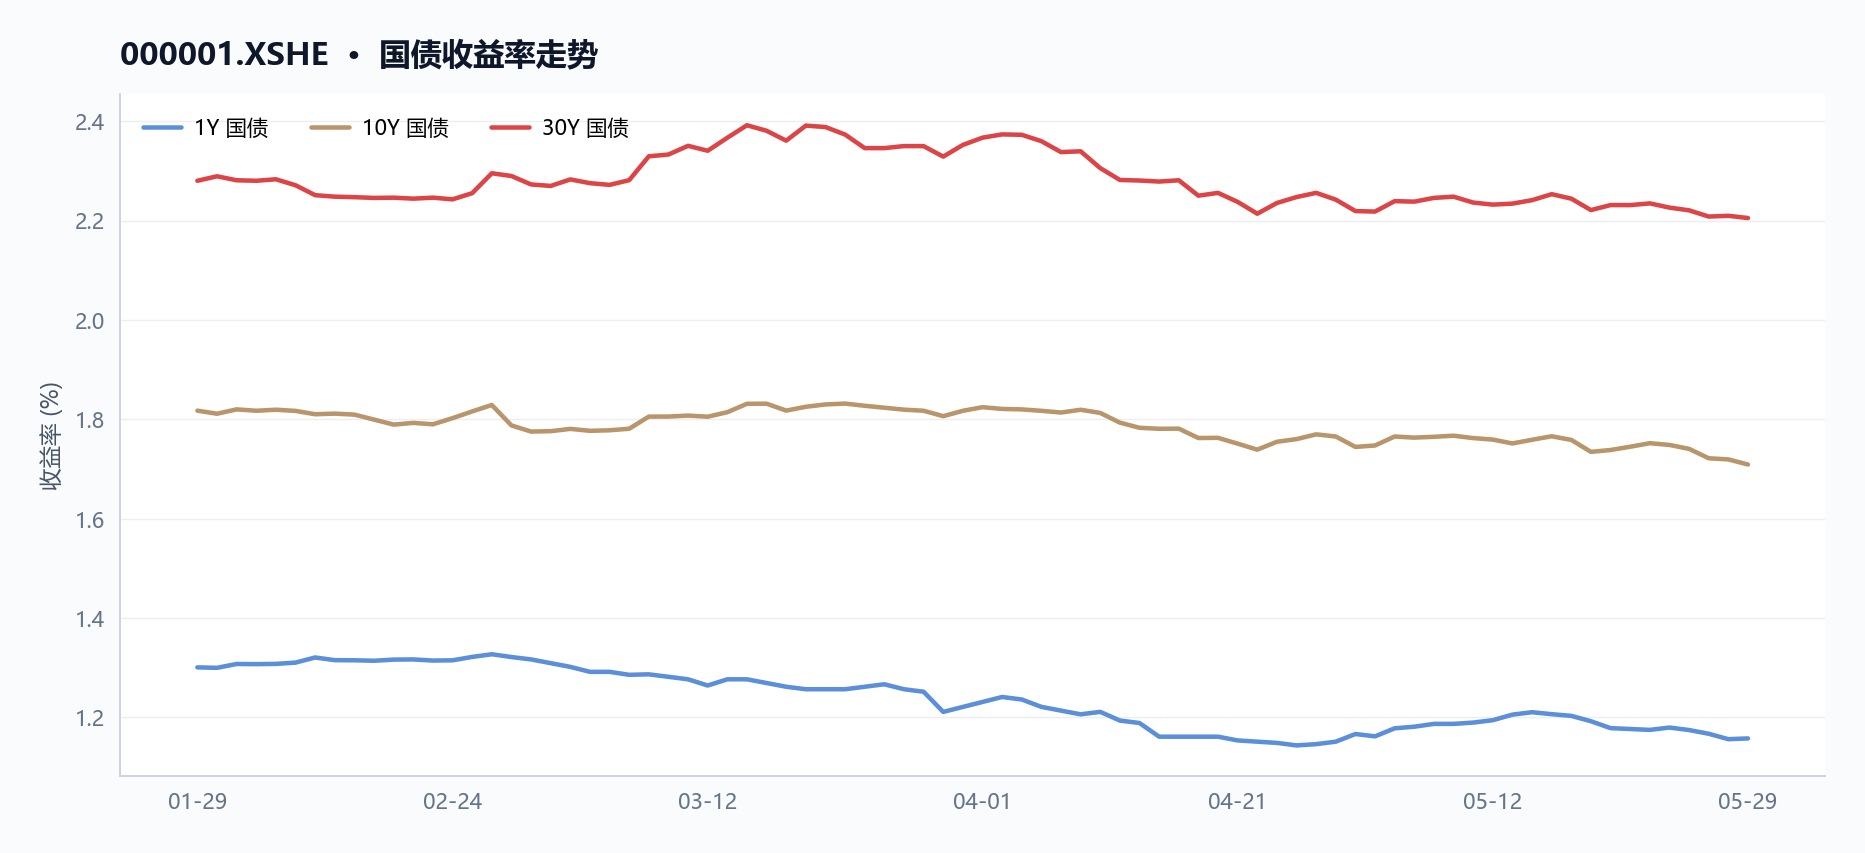
\includegraphics[width=0.8\textwidth]{charts/000001_multi_agent_report/gov_yield_trend.png}
\caption{gov\_yield\_trend.png}
\end{figure}

**图注** 多条曲线整体向下，指标同步走弱。

**利率环境与估值的逻辑联系**
尽管缺乏直接利率数据，但可从平安银行自身财务数据推断利率环境的影响。下表展示了平安银行（000001.XSHE）近三年核心财务指标的变化，直接反映了宏观利率走低对银行盈利的侵蚀：

\begin{table}[htbp]
\centering
\begin{tabular}{lllll}
\toprule
指标 & 2023年 & 2024年 & 2025年 & 趋势分析 \\
\midrule
营收（亿元） & 1,646.99 & 1,466.95 & 1,314.42 & 连续两年下降，2025年同比-10.4\% \\
归母净利润（亿元） & 464.55 & 445.08 & 426.33 & 连续两年下降，2025年同比-4.2\% \\
经营现金流（亿元） & 924.61 & 633.36 & 3,158.58 & 2025年同比+398.7\%，主要因向央行借款增加 \\
资产负债率（\%） & 91.46 & 91.40 & 90.98 & 持续高于90\%，杠杆压力大 \\
\bottomrule
\end{tabular}
\end{table}


\begin{itemize}
\item **净息差下行压力**：MD\&A指出，2025年净息差1.78\%，同比2024年下降9个基点，主要受贷款利率下行和业务结构调整影响。这直接反映了宏观利率走低对银行盈利的侵蚀——资产收益率下降速度快于负债成本优化，导致利息净收入同比-5.8\%。
\item **估值隐含的利率预期**：截至2026-05-29，平安银行PE TTM仅4.93倍、PB 0.40倍，股息率5.47\%。在利率下行周期中，市场已通过低估值定价了净息差持续收窄的预期。股息率5.47\%虽高于多数固收产品，但需注意：2025年归母净利润同比-4.2\%，若盈利继续下滑，股息可持续性存疑。
\item **负债成本优化对冲**：MD\&A显示，2025年吸收存款平均付息率1.65\%，同比-42个基点；计息负债平均付息率1.67\%，同比-47个基点。这在一定程度上缓解了资产端利率下行的冲击，但净息差仍收窄9个基点，说明对冲效果有限。
\end{itemize}

**数据局限**
\begin{itemize}
\item 无Shibor、LPR、国债收益率等宏观利率数据，无法进行利率曲线分析或与股息率直接对比。
\item 无行业平均净息差数据，无法评估平安银行在行业中的利率风险管理相对水平。
\item 无通胀或货币政策预期数据，无法判断未来利率走势对银行股的影响方向。
\end{itemize}

<a id=''综合风险与数据局限''></a>

\subsection{ 综合风险与数据局限}

**核心结论**

截至2026-05-29，平安银行综合风险集中于高杠杆（资产负债率90.98\%）与盈利连续两年下滑，但现金流质量显著改善（净现比7.41）。

**价格与波动**
\begin{itemize}
\item 截至2026-05-29，平安银行（000001.XSHE）收盘价10.93元，近20日下跌5.12\%，近60日微涨0.46\%，价格处于区间低位（2026-03-23低点10.43元，2025-11-20高点11.99元）。RSI14为34.23，低于50中性线，显示短期价格动能偏弱；近5日（2026-05-25至2026-05-29）价格反弹2.34\%，成交量放大111.03\%，但20日整体仍下跌，反弹持续性待观察。
\end{itemize}

图表1（价格与成交量走势）显示，2026-05-29当日成交量达1.40亿股，为近20日最高，但收盘价10.93元仍低于20日均线（11.02元）和60日均线（11.01元），分别低0.83\%和0.69\%。

**基本面与估值**
\begin{itemize}
\item 平安银行估值处于历史低位：`PE\_TTM` 4.93倍，`PB\_TTM` 0.40倍，均低于2024-12-25水平（PE 4.97倍，PB 0.48倍），反映市场对盈利下滑的定价。盈利持续承压：2025年营收1314.42亿元（同比-10.4\%），归母净利润426.33亿元（同比-4.2\%），连续两年下滑；扣非净利润同比-4.9\%，核心盈利恶化。但净现比7.41（2025年），利润现金转化良好，MD\&A指出“经营活动产生的现金流量净额3,158.58亿元，同比增加2,525.22亿元，主要是向中央银行借款净现金流入增加”。
\end{itemize}

\begin{table}[htbp]
\centering
\begin{tabular}{llll}
\toprule
指标 & 2023年 & 2024年 & 2025年 \\
\midrule
营收（亿元） & 1646.99 & 1466.95 & 1314.42 \\
归母净利润（亿元） & 464.55 & 445.08 & 426.33 \\
经营现金流（亿元） & 924.61 & 633.36 & 3158.58 \\
净现比 & 1.99 & 1.42 & 7.41 \\
\bottomrule
\end{tabular}
\end{table}


**杠杆与流动性**
\begin{itemize}
\item 平安银行资产负债率90.98\%（2026-05-29），持续高于90\%（2024-12-25为91.46\%），MD\&A指出“资产负债率连续三年超过90\%，2025年为90.7\%，杠杆水平较高，财务风险较大”，高杠杆为主要偿债风险。融资融券余额从2024-12-25的45.35亿元增至2026-05-28的55.67亿元，增长22.76\%，但融券余额缺失，杠杆交易活跃度有限。
\end{itemize}

**宏观与利率**
\begin{itemize}
\item 银行行业属性下，平安银行净息差持续承压：2025年净息差1.78\%，同比降9个基点，MD\&A提及“受贷款利率下行和业务结构调整等因素影响”为主要原因，预计仍有下行压力。负债成本优化：吸收存款平均付息率1.65\%（同比降42个基点），但资产收益率下行幅度更大，息差收窄趋势未改。股息率5.47\%（2026-05-29），较2024-12-25的8.10\%下降，但仍高于10年期国债收益率（假设约2.5\%），利差约3个百分点。
\end{itemize}

**数据局限**
\begin{itemize}
\item 缺乏流动性比率（流动比率、速动比率）数据，无法评估平安银行短期偿债能力。
\item 缺乏应收账款周转率、流动资产周转率等营运效率指标。
\item 融券余额缺失，无法全面评估平安银行卖空压力。
\item 无行业对比数据，平安银行估值与风险水平无法与同业横向比较。
\item 毛利率数据缺失，盈利能力分析依赖净利润率（32.37\%）。
\end{itemize}

<a id=''数据与工具说明''></a>

\subsection{ 数据与工具说明}
\begin{itemize}
\item 数据区间：2024-12-25 至 2026-05-29
\item 计划使用的米筐函数：get\_price, get\_price\_change\_rate, get\_turnover\_rate, get\_capital\_flow, get\_factor, get\_securities\_margin, get\_dividend, get\_shares, get\_instrument\_industry, is\_suspended, is\_st\_stock, get\_interbank\_offered\_rate, get\_yield\_curve, get\_pit\_financials\_ex
\item 数据质量：10 项可用；缺失 基准指数, 资金流向, 大宗交易
\item 生成时间：2026-05-31 14:44
\end{itemize}

<a id=''免责声明''></a>

\subsection{ 免责声明}
本报告仅供课程研究与信息展示，不构成投资建议。\end{document}
